% !TEX root = task-1-12-2.tex
% Editable task bank. Append new BankTask blocks at the end of the document.
\documentclass[12pt,a4paper]{article}
\usepackage{physics-textbook}
\usepackage{graphicx,needspace}
\usetikzlibrary{decorations.pathmorphing}
\newif\ifShowSolutions
\ifdefined\TutorEdition
  \ShowSolutionstrue
\else
  \ShowSolutionsfalse % Change to \ShowSolutionstrue to display solutions.
\fi
\newcounter{banktask}
\newsavebox{\BankTaskBox}
\newcommand{\BankTaskContent}[3]{%
  \noindent\textbf{\thebanktask.}\quad #2\par
  \ifShowSolutions
    \Needspace{50mm}% Keep the solution heading with its opening text or diagram.
    #3\par
    \ifdefined\TutorEdition
      \ifcsname TutorSource#1\endcsname
        \nopagebreak\smallskip{\small\csname TutorSource#1\endcsname\par}%
      \fi
    \fi
  \fi
}
\newcommand{\BankTask}[3]{%
  \refstepcounter{banktask}\par\medskip
  \sbox{\BankTaskBox}{\begin{minipage}{\linewidth}%
    \BankTaskContent{#1}{#2}{#3}\end{minipage}}%
  \ifdim\dimexpr\ht\BankTaskBox+\dp\BankTaskBox\relax>\dimexpr\textheight-20mm\relax
    \Needspace{35mm}\BankTaskContent{#1}{#2}{#3}%
  \else
    \Needspace{\dimexpr\ht\BankTaskBox+\dp\BankTaskBox\relax}%
    \noindent\usebox{\BankTaskBox}\par
  \fi
  \medskip
}
\begin{document}
\BookSubsection{1.12.2}{Условия равновесия}


% Source sdamgia-50713: https://phys-ege.sdamgia.ru/problem?id=50713
\BankTask{sdamgia-50713}{
Невесомый рычаг находится в равновесии. Левое плечо рычага равно $6 \,\text{см}$, правое плечо равно $15 \,\text{см}$. На правом плече подвешен груз массой $0{,}2 \,\text{кг}$. Какой массы груз нужно подвесить на левом плече, чтобы рычаг оставался в равновесии?
}{
\smallskip\noindent\textbf{Решение}\par
По правилу моментов $m_{1}g l_{1}=m_{2}g l_{2},$ откуда масса груза на левом плече равна

$m_{1}= \frac{ m_{2}l_{2}}{ l_{1} } = \frac{ 0{,}2 \cdot 15}{ 6 } =0{,}5\,\text{кг}.$

Ответ: $0{,}5$.
}

% Source sdamgia-35321: https://phys-ege.sdamgia.ru/problem?id=35321
\BankTask{sdamgia-35321}{
\begin{center}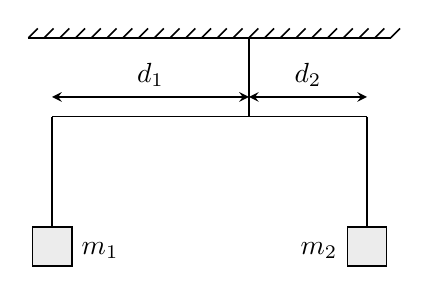
\begin{tikzpicture}[x=1cm,y=1cm,>=stealth,line width=.55pt]
\draw (-.3,2.7)--(4.3,2.7);\foreach \x in {-.3,-.1,...,4.3}{\draw(\x,2.7)--++(.12,.12);}\draw(2.5,2.7)--(2.5,1.7);\draw(0,1.7)--(4,1.7);\draw(0,1.7)--(0,.3);\draw(4,1.7)--(4,.3);\draw[fill=gray!15](-.25,-.2)rectangle(.25,.3);\draw[fill=gray!15](3.75,-.2)rectangle(4.25,.3);\node[right]at(.25,0){$m_1$};\node[left]at(3.75,0){$m_2$};\draw[<->](0,1.95)--(2.5,1.95)node[midway,above]{$d_1$};\draw[<->](2.5,1.95)--(4,1.95)node[midway,above]{$d_2$};
\end{tikzpicture}\end{center}
Коромысло весов, к которому подвешены на нитях два груза (см. рис.), находится в равновесии. Массу первого груза увеличили в $2$ раза. Во сколько раз нужно уменьшить плечо $d_{1}$, чтобы равновесие сохранилось? (Коромысло и нити считать невесомыми.)
}{
\smallskip\noindent\textbf{Решение}\par
Рычаг находится в равновесии, если моменты приложенных сил равны. Поскольку плечо второй силы и массу второго груза не меняли, то момент этой силы не изменился. Соответственно, момент первой силы также остался прежним. Поскольку момент силы равен $M=m_{1}gd_{1},$ масса груза увеличилась в $2$ раза, то плечо силы необходимо уменьшить в $2$ раза.
 
Ответ: $2$.
}

% Source sdamgia-35987: https://phys-ege.sdamgia.ru/problem?id=35987
\BankTask{sdamgia-35987}{
К концу тонкого жесткого однородного стержня длиной $50 \,\text{см}$ и массой $300 \,\text{г}$ прикреплен маленький шарик массой $200 \,\text{г}$. На каком расстоянии от шарика нужно поставить под него тонкую опору, чтобы эта система тел находилась в равновесии в однородном поле силы тяжести?
}{
\smallskip\noindent\textbf{Решение}\par
Рычаг находится в равновесии, если моменты приложенных сил равны. Пусть плечо силы, действующей на рычаг со стороны шарика, равно $x$. Тогда плечо силы тяжести однородного стрежня равно $\frac{ l}{ 2 } - x.$ По правилу моментов рычаг находится в равновесии, если выполняется условие:

$mg ( \frac{ l}{ 2 } - x ) = m_{1}gx,$

откуда находим расстояние от точки опоры до маленького шарика:

$x= \frac{ ml}{ 2 ( m + m_{1} ) } = \frac{ 300 \cdot 50}{ 2 ( 300 + 200 ) } =15\,\text{см}.$

Ответ: $15$.
}

% Source sdamgia-27973: https://phys-ege.sdamgia.ru/problem?id=27973
\BankTask{sdamgia-27973}{
Однородный стержень массой $m=48 \,\text{кг}$ подвешен в горизонтальном положении на двух канатах так, как показано на рисунке. Каждый из канатов составляет с вертикалью угол $\alpha =60 ^\circ.$ Найдите модуль силы натяжения каждого из канатов.

\begin{center}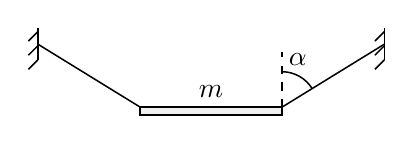
\begin{tikzpicture}[x=1cm,y=1cm,>=stealth,line width=.55pt]
\draw (0,1.3)--(0,1.7);\foreach \y in {1.3,1.48,...,1.7}{\draw (0,\y)--++(-.12,-.12);}\draw (4.4,1.3)--(4.4,1.7);\foreach \y in {1.3,1.48,...,1.7}{\draw (4.4,\y)--++(-.12,-.12);}\draw (0,1.5)--(1.3,.7);\draw (3.1,.7)--(4.4,1.5);\draw[fill=gray!12] (1.3,.6) rectangle (3.1,.7);\node[above] at (2.2,.7){$m$};\draw[dashed] (3.1,.7)--(3.1,1.4);\draw (3.1,1.15) arc (90:31:.45);\node at (3.3,1.3){$\alpha$};
\end{tikzpicture}\end{center}
}{
\smallskip\noindent\textbf{Решение}\par
Изобразим силы, действующие на стержень:

\begin{center}\begin{tikzpicture}[x=1cm,y=1cm,>=stealth,line width=.55pt]
\draw (0,1.3)--(0,1.7);\foreach \y in {1.3,1.48,...,1.7}{\draw (0,\y)--++(-.12,-.12);}\draw (4.4,1.3)--(4.4,1.7);\foreach \y in {1.3,1.48,...,1.7}{\draw (4.4,\y)--++(-.12,-.12);}\draw (0,1.5)--(1.3,.7);\draw (3.1,.7)--(4.4,1.5);\draw[fill=gray!12] (1.3,.6) rectangle (3.1,.7);\node[above] at (2.2,.7){$m$};\draw[dashed] (3.1,.7)--(3.1,1.4);\draw (3.1,1.15) arc (90:31:.45);\node at (3.3,1.3){$\alpha$};\draw[->] (1.3,.7)--(.45,1.22) node[above]{$\vec F_{\text{н}1}$};\draw[->] (3.1,.7)--(3.95,1.22) node[above]{$\vec F_{\text{н}2}$};\draw[->] (2.2,.65)--(2.2,-.45) node[below]{$m\vec g$};
\end{tikzpicture}\end{center}

Запишем условие равновесия невращающегося тела:
$m\vec{g} + \vec{F}_{\text{н1}} + \vec{F}_{\text{н2}}=0;$
$Ox: F_{\text{н1}} \sin \alpha - F_{\text{н2}} \sin \alpha =0 \Rightarrow F_{\text{н1}}=F_{\text{н2}}=F_{\text{н}};$
$Oy: 2F_{\text{н}} \cos \alpha - mg=0.$
 
Откуда следует, что:

$F_{\text{н}}= \frac{ mg}{ 2 \cos \alpha } = \frac{ 48 \cdot 10}{ 2 \cdot 0{,}5 } =480\,\text{Н}.$

Ответ: $480$.
}

% Source sdamgia-10176: https://phys-ege.sdamgia.ru/problem?id=10176
\BankTask{sdamgia-10176}{
К горизонтальной легкой рейке, лежащей на двух опорах А и В, в точке О прикреплен груз массой $10 \,\text{кг}$. Длина отрезка ОА равна $4 \,\text{м}$, длина отрезка ОВ равна $1 \,\text{м}$. Определите модуль силы, с которой действует на рейку опора В.

\begin{center}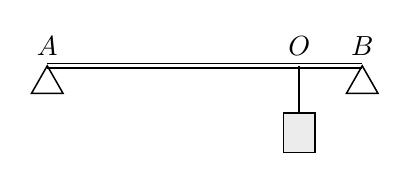
\begin{tikzpicture}[x=1cm,y=1cm,>=stealth,line width=.55pt]
\draw[double,double distance=1pt] (0,0)--(4,0);\draw (0,0)--(-.2,-.35)--(.2,-.35)--cycle;\draw (4,0)--(3.8,-.35)--(4.2,-.35)--cycle;\node[above] at(0,0){$A$};\node[above] at(4,0){$B$};\node[above] at(3.2,0){$O$};\draw (3.2,0)--(3.2,-.6);\draw[fill=gray!15] (3,-1.1) rectangle (3.4,-.6);
\end{tikzpicture}\end{center}
}{
\smallskip\noindent\textbf{Решение}\par
На рейку действуют сила реакции опоры в точке $A$ и в точке $B$, а также сила тяжести груза. Запишем уравнение моментов относительно точки А:

$mg \cdot OA=N_{B} \cdot AB \Rightarrow N_{B} = \frac{ mg \cdot OA}{ AB } = \frac{ 10 \cdot 10 \cdot 4}{ 5 } =80\,\text{Н}.$

Ответ: $80$.
}

% Source sdamgia-10309: https://phys-ege.sdamgia.ru/problem?id=10309
\BankTask{sdamgia-10309}{
К легкой рейке подвешено на нити тело массой $7 \,\text{кг}$ (см. рис.). Рейка уравновешена на шероховатой опоре в горизонтальном положении с помощью силы $\vec{F},$ приложенной к концу рейки и направленной под углом $\alpha=30 ^\circ$ к горизонту. Определите модуль вертикальной составляющей силы реакции опоры, действующей на рейку в точке $O$.

\begin{center}\begin{tikzpicture}[x=1cm,y=1cm,>=stealth,line width=.55pt]
\draw[double,double distance=1pt] (0,0)--(5.6,0);\foreach \i in {0,...,14}{\fill (.4*\i,0) circle(1pt);}\draw (2.8,0)--(2.6,-.35)--(3,-.35)--cycle;\node[above] at(2.8,.1){$O$};\draw (1.6,0)--(1.6,-.7);\draw[fill=gray!15] (1.4,-1.15) rectangle (1.8,-.7);\node[below] at(1.6,-1.15){$7\,\text{кг}$};\draw[->] (0,0)--(-1,.58) node[above]{$\vec F$};\draw (-.6,0) arc(180:150:.6);\draw(-.9,0)--(0,0);\node at(-.7,.2){$\alpha$};
\end{tikzpicture}\end{center}
}{
\smallskip\noindent\textbf{Решение}\par
Так как рейка уравновешена, запишем правило моментов относительно левого края рейки, тем самым исключив силу $F$:

$Nd_{1}=mgd_{2} \Longleftrightarrow N= \frac{ mgd_{2}}{ d_{1} } = \frac{ 70 \cdot 4}{ 7 } =40\,\text{Н}.$

Ответ: $40$.
}

% Source sdamgia-3704: https://phys-ege.sdamgia.ru/problem?id=3704
\BankTask{sdamgia-3704}{
\begin{center}\begin{tikzpicture}[x=1cm,y=1cm,>=stealth,line width=.55pt]
\draw (4,0)--(4,3.3);\foreach \y in {0,0.18,...,3.3}{\draw (4,\y)--++(-.12,-.12);}\draw (1.2,2.6) circle (.3);\draw (2.2,2.3) circle (.3);\draw (3.2,2) circle (.3);\foreach \x/\y in {1.2/2.6,2.2/2.3,3.2/2}{\fill (\x,\y) circle(1pt);}\draw (1.2,2.9)--(4,2.9);\draw (1.2,2.3)--(2.2,2.3);\draw (2.2,2.6)--(4,2.6);\draw (2.2,2)--(3.2,2);\draw (3.2,2)--(4,2);\draw (3.5,2)--(3.5,.55);\draw[fill=gray!15] (3.3,0) rectangle (3.7,.55);\node[below] at (3.5,0){$10\,\text{кг}$};\draw[->] (1.2,2.6)--(-.5,2.6) node[above]{провод};
\end{tikzpicture}\end{center}
На железной дороге для натяжения проводов используется показанная на рисунке система, состоящая из легких блоков и тросов, натягиваемых тяжелым грузом. Чему равна сила натяжения провода? Трение в осях блоков мало. Блоки и нити считайте невесомыми.
}{
\smallskip\noindent\textbf{Решение}\par
\begin{center}\begin{tikzpicture}[x=1.6cm,y=1.7cm,>=stealth,line width=.55pt]
\draw (4,0)--(4,3.3);\foreach \y in {0,0.18,...,3.3}{\draw (4,\y)--++(-.12,-.12);}\draw (1.2,2.6) circle (.3);\draw (2.2,2.3) circle (.3);\draw (3.2,2) circle (.3);\foreach \x/\y in {1.2/2.6,2.2/2.3,3.2/2}{\fill (\x,\y) circle(1pt);}\draw (1.2,2.9)--(4,2.9);\draw (1.2,2.3)--(2.2,2.3);\draw (2.2,2.6)--(4,2.6);\draw (2.2,2)--(3.2,2);\draw (3.2,2)--(4,2);\draw (3.5,2)--(3.5,.55);\draw[fill=gray!15] (3.3,0) rectangle (3.7,.55);\node[below] at (3.5,0){$10\,\text{кг}$};\draw[->] (1.2,2.6)--(-.5,2.6) node[above]{провод};\draw[->] (1.2,2.6)--(.1,2.6) node[below]{$4\vec T$};\draw[->] (1.2,2.9)--(2,2.9) node[above]{$2\vec T$};\draw[->] (1.2,2.3)--(1.9,2.3);\draw[->] (2.2,2.6)--(3,2.6) node[above]{$\vec T$};\draw[->] (2.2,2)--(2.9,2);\draw[->] (3.5,.55)--(3.5,-.8) node[below]{$m\vec g$};
\draw[->] (3.5,.55)--(3.5,1.35) node[right]{$\vec T$};\draw[->] (2.2,2.3)--(1.3,2.3) node[midway,above]{$2\vec T$};\node[above] at (2.8,3.55){вторая нить};\node[align=center] at (-.45,1.7){подвижные\\блоки};\draw (-.1,1.95)--(.98,2.42);\draw (-.1,1.6)--(1.95,2.2);\node[align=center] at (.2,.7){первая нить};\draw (.7,.85)--(2.4,2.6);\node[align=center] at (1.55,-.25){неподвижный\\блок};\draw (2,.1)--(3.05,1.8);\end{tikzpicture}\end{center}

Система, представленная на рисунке, состоит из трех блоков: двух подвижных и одного неподвижного. Назначение неподвижного блока заключается только в том, что он меняет направление действия силы, однако никакого выигрыша в силе при этом не возникает. Каждый подвижный блок, напротив, дает выигрыш в силе.
Определим силу, с которой натянута первая нить. Груз растягивает ее с силой:

$T=mg=10\,\text{кг} \cdot 10\,\text{м}/\,\text{с} ^{2} =100\,\text{Н}.$ 

Рассмотрим теперь первый подвижный блок. Поскольку вся система статична, полная сила, действующая на этот блок, должна быть равна нулю. Первая нить тянет его направо с суммарной силой $2T,$ значит, натяжение второй нити тоже должно быть равно $2T$ (вот он — выигрыш в силе). Аналогичное рассмотрение для второго подвижного блока показывает, что натяжение провода должно быть равно $4T=4 \cdot 100\,\text{Н}=400\,\text{Н}.$
 
Ответ: $400$.
}

% Source sdamgia-9099: https://phys-ege.sdamgia.ru/problem?id=9099
\BankTask{sdamgia-9099}{
Однородная лестница массой $20 \,\text{кг}$ прислонена к гладкой вертикальной стене, составляя с ней угол $60^\circ$. Пол шероховатый. Чему равен модуль силы реакции, действующей на верхний конец лестницы?
}{
\smallskip\noindent\textbf{Решение}\par
\begin{center}\begin{tikzpicture}[x=1cm,y=1cm,>=stealth,line width=.55pt]
\draw[->](0,0)--(3.8,0)node[right]{$x$};\draw[->](0,0)--(0,2.5)node[above]{$y$};\draw(0,1.8)--(3.12,0);\node[below]at(3.12,0){$O$};\draw[->](0,1.8)--(1,1.8)node[above]{$\vec N_1$};\draw[->](3.12,0)--(3.12,1.1)node[right]{$\vec N_2$};\draw[->](3.12,0)--(2,0);\node[anchor=north] at (2.55,-.16){$\vec F_{\text{тр}}$};\draw[->](1.56,.9)--(1.56,-.1);\node[anchor=north east] at (1.47,-.15){$m\vec g$};\draw(0,1.2)arc(-90:-30:.6);\node at(.35,1.1){$60^\circ$};
\end{tikzpicture}\end{center}

Запишем правило моментов, взяв за ось вращения точку $O$, а за длину лестницы $l$:

$N_{1}l \cos \alpha =mg \frac{ l}{ 2 } \sin \alpha .$

Выразим модуль силы реакции, действующей на верхний конец лестницы:

$N_{1}= \frac{ mg \tan \alpha }{ 2 } = \frac{ 20 \cdot 10 \cdot \sqrt{3} }{ 2 } \approx 173\,\text{Н}.$

Ответ: $173 \,\text{Н}$.
}

% Source sdamgia-39935: https://phys-ege.sdamgia.ru/problem?id=39935
\BankTask{sdamgia-39935}{
\begin{center}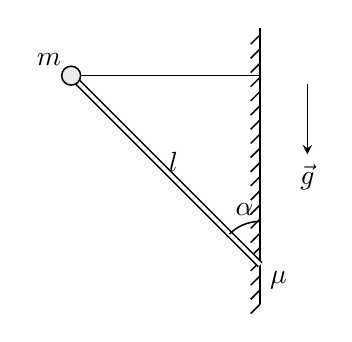
\begin{tikzpicture}[x=1cm,y=1cm,>=stealth,line width=.55pt]
\draw (2.8,0)--(2.8,3.5);\foreach \y in {0,0.18,...,3.5}{\draw (2.8,\y)--++(-.12,-.12);}\draw[double,double distance=1.4pt] (.4,2.9)--(2.8,.5);\draw (.4,2.9)--(2.8,2.9);\draw[fill=gray!15] (.4,2.9) circle (.12);\node[above left] at (.4,2.9){$m$};\node at (1.7,1.8){$l$};\draw (2.8,1.05) arc (90:135:.55);\node at (2.6,1.2){$\alpha$};\node[right] at (2.8,.3){$\mu$};\draw[->] (3.4,2.8)--(3.4,1.9) node[below]{$\vec g$};
\end{tikzpicture}\end{center}
Маленький шарик массой $m$ закреплён на верхнем конце тонкого лёгкого стержня длиной $l$, нижний конец которого упирается в шероховатую вертикальную стену с коэффициентом трения, равным $\mu = 0{,}5,$ а верхний соединён горизонтальной невесомой нерастяжимой нитью со стеной (см. рисунок). Система находится в равновесии. Каков может быть при этом угол $\alpha$ между стержнем и стеной?
}{
\smallskip\noindent\textbf{Решение}\par
\begin{center}\begin{tikzpicture}[x=1cm,y=1cm,>=stealth,line width=.55pt]
\draw (2.8,0)--(2.8,3.5);\foreach \y in {0,0.18,...,3.5}{\draw (2.8,\y)--++(-.12,-.12);}\draw[double,double distance=1.4pt] (.4,2.9)--(2.8,.5);\draw (.4,2.9)--(2.8,2.9);\draw[fill=gray!15] (.4,2.9) circle (.12);\node[above left] at (.4,2.9){$m$};\node at (1.7,1.8){$l$};\draw (2.8,1.05) arc (90:135:.55);\node at (2.6,1.2){$\alpha$};\node[right] at (2.8,.3){$\mu$};\draw[->] (3.4,2.8)--(3.4,1.9) node[below]{$\vec g$};\draw[->] (.4,2.9)--(1.8,2.9) node[above]{$\vec T$};\draw[->] (.4,2.9)--(.4,1.7) node[left]{$m\vec g$};\draw[->] (2.8,.5)--(1.8,.5) node[below]{$\vec N$};\draw[->] (2.8,.5)--(2.8,1.8) node[left]{$\vec F_{\text{тр}}$};
\end{tikzpicture}\end{center}

\par\smallskip\noindent $1$. Изобразим силы, действующие на стержень с шариком на конце (см. рисунок): это сила тяжести $m \vec{g},$ сила натяжения нити $\vec{T},$ сила $\vec{N}$ реакции стены и сила $\vec{F}_{\text{тр}}$ трения конца стержня о стену $( F_{\text{тр}} \le \mu N ) .$ 
\par\smallskip\noindent $2$. Из условий равновесия твёрдого тела в ИСО следует равенство нулю сумм проекций сил на вертикаль и на горизонталь, действующих на стержень с шариком, а также моментов этих сил относительно оси, проходящей через нижний конец стержня: 

$T = N,$
$mg = F_{\text{тр}} \le \mu N,$
$T \cdot l \cos \alpha = mg \cdot l \sin \alpha .$

\par\smallskip\noindent $3$. Решая данную систему уравнений, получаем: $\tan \alpha \ge \frac{ 1}{ \mu } = 2,$ $\alpha \ge 63{,}4 ^\circ.$
 
Ответ: $\arctan \frac{ 1}{ \mu } \le \alpha < 90 ^\circ,$ $63{,}4 ^\circ \le \alpha < 90 ^\circ.$
}

% Source sdamgia-3418: https://phys-ege.sdamgia.ru/problem?id=3418
\BankTask{sdamgia-3418}{
Однородную балку поднимают за один конец, прикладывая силу $\vec{F}$ перпендикулярно балке. На рисунке показан график изменения модуля силы по мере подъема конца балки. 

 

\begin{center}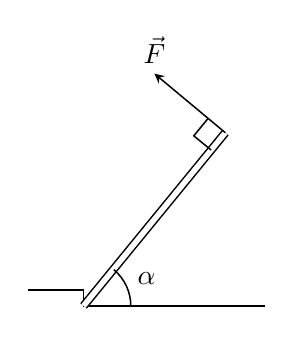
\begin{tikzpicture}[x=1cm,y=1cm,>=stealth,line width=.55pt]
\draw (-.7,0)--(0,0)--(0,-.2)--(2.3,-.2);\draw[double,double distance=2pt] (0,-.2)--(1.8,2);\draw[->] (1.8,2)--(.9,2.75) node[above]{$\vec F$};\draw (1.62,1.78)--(1.4,1.96)--(1.58,2.18);\draw (.6,-.2) arc(0:50:.6);\node at (.8,.15){$\alpha$};
\end{tikzpicture}\end{center}

\begin{center}\begin{tikzpicture}[x=1cm,y=1cm,>=stealth,line width=.55pt]
\draw[step=.5,gray!50,thin] (0,0) grid (3,3);\draw[->] (-.25,0)--(3.4,0) node[right]{$\alpha,\ \text{рад}$};\draw[->] (0,-.25)--(0,3.35) node[above]{$F,\ \text{Н}$};\draw[thick] (0,2) arc(90:0:2);\foreach \y/\v in {.5/100,1/200,1.5/300,2/400}{\node[left] at(0,\y){$\v$};}\node[below left] at(0,0){$0$};\node[below] at(2,0){$\pi/2$};
\end{tikzpicture}\end{center}

Чему равна масса балки?
}{
\smallskip\noindent\textbf{Решение}\par
Проще всего определить массу балки, рассмотрев самое начало подъема. Для того чтобы правый конец балки начал подниматься, вращающий момент, создаваемый силой $\vec{F}$ относительно левого конца балки, должен стать больше момента, создаваемого силой тяжести относительно этой точки. Сила тяжести приложена к центру масс балки. Поскольку балка однородная, ее центр масс расположен посередине. Обозначим длину балки через $L.$ По правилу моментов приложенных сил $Mg \frac{ L}{ 2 } =FL.$ 
Следовательно, масса балки равна $M= \frac{ 2F}{ g } .$ Из графика видно, что в самом начале для подъема балки была необходима сила в $400 \,\text{Н}$. Следовательно, масса балки равна $M=\frac{2\cdot400}{10}=80\,\text{кг}$.
 
Ответ: $80 \,\text{кг}$.
}


% Source 51276: https://phys-ege.sdamgia.ru/problem?id=51276
\BankTask{51276}{
\begin{center}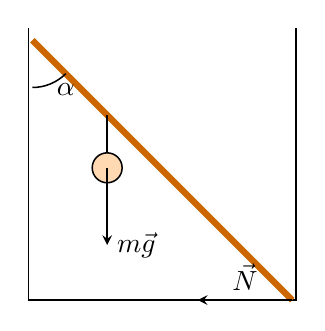
\begin{tikzpicture}[>=stealth,line width=.55pt]\draw(-.05,3.45)--(-.05,0)--(3.35,0)--(3.35,3.45);\draw[orange!80!black,line width=2.3pt](0,3.3)--(3.3,0);\draw(0,2.7)arc(-90:-45:.6)node[below]{$\alpha$};\draw(.95,2.35)--(.95,1.68);\draw[fill=orange!30](.95,1.68)circle(.19);\draw[->](.95,1.68)--(.95,.7)node[right]{$m\vec g$};\draw[->](3.3,0)--(2.1,0)node[midway,above]{$\vec N$};\end{tikzpicture}\end{center}Невесомый стержень длиной $4\,\text{м}$, находящийся в ящике с гладкими дном и стенками, составляет с вертикалью угол $\alpha$  =  $30$° (см. рис.). К стержню на некотором расстоянии от верхнего конца подвешен на нити шар массой $2\,\text{кг}$. Модуль силы нормальной реакции правой стенки ящика, действующей на нижний конец стержня, равен N  =  $7{,}5$ Н. На каком расстоянии x от верхнего конца стержня подвешен шар?
}{
\smallskip\noindent\textbf{Решение}\par
\begin{center}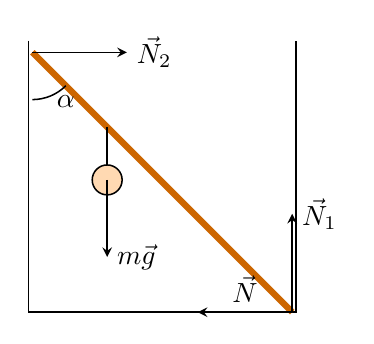
\begin{tikzpicture}[>=stealth,line width=.55pt]\draw(-.05,3.45)--(-.05,0)--(3.35,0)--(3.35,3.45);\draw[orange!80!black,line width=2.3pt](0,3.3)--(3.3,0);\draw(0,2.7)arc(-90:-45:.6)node[below]{$\alpha$};\draw(.95,2.35)--(.95,1.68);\draw[fill=orange!30](.95,1.68)circle(.19);\draw[->](.95,1.68)--(.95,.7)node[right]{$m\vec g$};\draw[->](3.3,0)--(2.1,0)node[midway,above]{$\vec N$};\draw[->](0,3.3)--(1.2,3.3)node[right]{$\vec N_2$};\draw[->](3.3,0)--(3.3,1.25)node[right]{$\vec N_1$};\end{tikzpicture}\end{center}Изобразим силы, действующие на стержень. Для абсолютно твердого тела, каким можно считать стержень, можно применить два условия равновесия:

\[\overrightarrow{N}_2 + \overrightarrow{N}_1 + \overrightarrow{N} + m \vec{g} = 0,\]

где $\overrightarrow{N}_2$  — реакция левой стенки, действующая на верхний конец, $\overrightarrow{N}_1$  —  реакция дна, действующая на верхний конец, $\overrightarrow{N}$  — реакция правой стенки. 
В проекции на горизонтальную ось:

$N_2 - N = 0,$
то есть
$N_2=N.$

Применим правило моментов сил относительно оси, проходящей через нижнюю точку стержня в точке её касания стенки:

\[mg \cdot ( L - x ) \sin \alpha - N_2 L \cos \alpha = 0.\]

Тогда искомое расстояние:

\[x = ( 1 - \frac{N}{mg \cdot \tan \alpha} ) \cdot L = 4 \,\text{м} \cdot ( 1 - \frac{7{,}5 \,\text{Н}}{2 \,\text{кг} \cdot 10 \,\text{м/с} ^2 \cdot \tfrac{1}{\sqrt{3}}} ) = 1{,}4 \,\text{м}.\]

Ответ: $1{,}4\,\text{м}$.
}

% Source 25744: https://phys-ege.sdamgia.ru/problem?id=25744
\BankTask{25744}{
Два небольших шара массами $m_{1}$ = $0{,}2\,\text{кг}$ и $m_{2}$ = $0{,}3\,\text{кг}$ закреплены на концах невесомого стержня $AB$, расположенного горизонтально на опорах $C$ и $D$ (см. рис.). Расстояние между опорами l = $0{,}6\,\text{м}$, а расстояние $AC$ равно $0{,}2\,\text{м}$. Чему равна длина стержня $L$, если сила давления стержня на опору $D$ в $2$ раза больше, чем на опору $C$? Сделайте рисунок с указанием внешних сил, действующих на систему тел «стержень  — шары».
Какие законы Вы используете для описания равновесия тела? Обоснуйте их применение к данному случаю.
\begin{center}\begin{tikzpicture}[task graph,>=stealth]
\draw(.5,1)rectangle(5.5,1.15);\draw(.5,.75)circle(.25)(5.5,.75)circle(.25);
\node[above]at(.5,1.15){$A$};\node[above]at(5.5,1.15){$B$};
\node[left]at(.25,.65){$m_1$};\node[right]at(5.75,.65){$m_2$};
\draw(1.8,0)--(2,1)--(2.2,0)--cycle;\draw(4.5,0)--(4.7,1)--(4.9,0)--cycle;
\node[left]at(2,.8){$C$};\node[left]at(4.7,.8){$D$};\draw(.2,0)--(5.8,0);
\foreach \x in {.4,.6,...,5.8}{\draw(\x,0)--++(-.12,-.12);}
\end{tikzpicture}\end{center}
}{
\smallskip\noindent\textbf{Решение}\par
Обоснование. Систему отчета, связанную с Землей, будем считать инерциальной. Для данной системы отсчета можно применить законы Ньютона (в частности, третий закон).
Тело, образованное стержнем и двумя шарами, будем считать абсолютно твердыми. Движение абсолютно твердого тела представляет собой суперпозицию поступательного и вращательного движений, поэтому для него можно применить условие равновесия для поступательного движения и правило моментов. Векторная сумма всех внешних сил, действующих на тело, равна нулю, поэтому сумма моментов этих сил относительно двух любых его параллельных осей одна и таже. Для удобства ось, относительно которой будем рассматривать сумму моментов сил, проведем перпендикулярно плоскости чертежа через точку А.

Перейдем к решению. На твердое тело, образованное стержнем и двумя шарами, действуют силы тяжести $m_1\vec g$ и $m_2\vec g,$ приложенные к центрам шаров, и силы реакции опор $\vec N_1$ и $\vec N_2.$ По третьему закону Ньютона, модули сил реакции равны соответствующим модулям сил давления стержня на опоры, поэтому $N_2 = 2N_1$ (в соответствии с условием задачи).
\begin{center}\begin{tikzpicture}[task graph,>=stealth]\draw[->](-.6,-.5)--(6,-.5)node[right]{$x$};\foreach \xx in {-.6,-.44,...,5.45}{\draw(\xx,-.5)--++(.12,-.12);}\draw[->](-.6,-1.8)--(-.6,2.1)node[above]{$y$};\node[below left]at(-.6,-.5){$O$};\draw[fill=gray!10](0,.55)rectangle(5,.7);\foreach\x/\l in{0/A,5/B}{\draw[fill=gray!15](\x,.3)circle(.2);\node[above]at(\x,.85){$\l$};}\foreach\x/\l in{1.4/C,4.2/D}{\draw(\x,.55)--++(-.2,-1.05)--++(.4,0)--cycle;\node[left]at(\x,.1){$\l$};}\node[right]at(.3,.2){$m_1$};\node[right]at(5.3,.2){$m_2$};\draw[->,thick](1.4,.55)--(1.4,1.6)node[above]{$\vec N_1$};\draw[->,thick](4.2,.55)--(4.2,2)node[above]{$\vec N_2$};\draw[->,thick](0,.3)--(0,-1.4)node[right]{$m_1\vec g$};\draw[->,thick](5,.3)--(5,-1.6)node[right]{$m_2\vec g$};\end{tikzpicture}\end{center}
В инерциальной системе отсчета $Oxy$, связанной с Землей, условия равновесия твердого тела приводят к набору уравнений:

\[N_1 + N_2 - m_1g - m_2g = 0\]

  — центр масс не движется вдоль оси $Oy$.

\[N_1x + N_2 ( l + x ) - m_2gL = 0\]

  — нет вращения вокруг оси, проходящей перпендикулярно рисунку через точку $A$.
 Здесь $x = AC = 0{,}2\,\text{м}$  — плечо силы реакции $N_{1}$.
 С учетом условия $N_2 = 2N_1$ уравнения приводятся к виду:

$3N_1 = ( m_1 + m_2 ) g,$
$( 3x + 2l ) N_1 = m_2gL.$

 Поделив второе уравнение на первое, получим:

\[L \frac{m_2}{m_1 + m_2} = x + \frac{2}{3} l.\]

 Откуда:

\[L = ( 1 + \frac{m_1}{m_2} ) \cdot ( x + \frac{2}{3} l ) = ( 1 + \frac{0{,}2\,\text{кг}}{0{,}3\,\text{кг}} ) \cdot ( 0{,}2\,\text{м} + \frac{2}{3} \cdot 0{,}6\,\text{м} ) = 1\,\text{м}.\]

Ответ: $1\,\text{м}$.
}

% Source 25722: https://phys-ege.sdamgia.ru/problem?id=25722
\BankTask{25722}{
\begin{center}\begin{tikzpicture}[task graph,>=stealth]
\draw(0,0)--(0,4.3);\draw(0,0)--(5,0);
\foreach \y in {0,.2,...,4.2}{\draw(0,\y)--++(-.12,-.12);}
\foreach \x in {0,.2,...,5}{\draw(\x,0)--++(-.12,-.12);}
\draw(.8,0)--(1.3,1)--(1.8,0)--cycle;
\draw[double,double distance=1.5pt](1.3,1)--(3.7,3.4);\draw(0,3.4)--(3.7,3.4);
\fill(1.3,1)circle(1.3pt)(3.7,3.4)circle(1.3pt);
\draw[dashed](1.3,1)--(4.5,1);\draw(2,1)arc(0:45:.7);
\node at(2.2,1.35){$\alpha$};\node[below left]at(1.3,1){$A$};\node[above right]at(3.7,3.4){$B$};\node[above left]at(0,3.4){$C$};
\end{tikzpicture}\end{center}Тонкий однородный стержень АВ шарнирно закреплен в точке А и удерживается горизонтальной нитью ВС (см. рис.). Трение в шарнире пренебрежимо мало. Масса стержня $m$  =  $1\,\text{кг}$, угол его наклона к горизонту $\alpha$ = $45$°. Найдите модуль силы $\vec F,$ действующей на стержень со стороны шарнира. Сделайте рисунок, на котором укажите все силы, действующие на стержень.
Какие законы Вы используете для описания равновесия стержня? Обоснуйте их применение к данному случаю.
}{
\smallskip\noindent\textbf{Решение}\par
Обоснование. Систему отсчета, связанную с Землей будем считать инерциальной. Стержень будем считать абсолютно твердым телом (формы и размеры тела неизменны, расстояние между любыми двумя его точками остается постоянным). Движение абсолютно твердого тела представляет собой суперпозицию поступательного и вращательного движений. Поэтому условия равновесия для него ровно два: одно для поступательного, а другое для вращательного движений. В инерциальной системе отсчета можно применить I условие равновесия покоящегося тела (векторная сумма всех сил, действующих на тело, равна нулю). Стержень является однородным, то есть имеет одинаковую плотность по всей длине. Поэтому центр тяжести стержня находится посередине. Ось, относительно которой будем рассматривать сумму моментов сил, проведем перпендикулярно плоскости чертежа через точку $A$

Перейдем к решению.
$1$.  Изобразим на рисунке силы, действующие на стержень, и систему координат Оху.
Здесь $\vec T$  — сила натяжения нити, $m\vec g$  — сила тяжести, $\vec F_x$ и $\vec F_y$  — вертикальная и горизонтальная составляющие силы, действующей на стержень со стороны шарнира.
\begin{center}\begin{tikzpicture}[task graph,>=stealth]\draw(0,0)--(0,4.5);\foreach \yy in {.2,.4,...,4.4}{\draw(0,\yy)--++(-.15,-.15);}\foreach \xx in {.2,.4,...,4.4}{\draw(\xx,0)--++(-.15,-.15);}\draw[->](0,0)--(4.5,0)node[right]{$x$};\draw[->](0,0)--(0,5)node[above]{$y$};\draw[very thick](1,.5)--(4,3.5);\draw(0,3.5)--(4,3.5);\draw(1,.5)--(.7,0)--(1.3,0)--cycle;\draw[dashed](1,.5)--(4.6,.5);\draw(1.7,.5)arc(0:45:.7)node[midway,right]{$\alpha$};\node[below left]at(1,.5){$A$};\node[right]at(4,3.5){$B$};\node[above right]at(0,3.5){$C$};\node[above left]at(2.5,2){$l$};\draw[->,thick](4,3.5)--(2.7,3.5)node[above]{$\vec T$};\draw[->,thick](1,.5)--(2.4,.5)node[below]{$\vec F_x$};\draw[->,thick](1,.5)--(1,1.9)node[left]{$\vec F_y$};\draw[->,thick](2.5,2)--(2.5,.8)node[right]{$m\vec g$};\end{tikzpicture}\end{center}
$2$.  В положении равновесия равна нулю сумма моментов сил, действующих на стержень, относительно оси, проходящей через точку А перпендикулярно плоскости рисунка, сумма горизонтальных и сумма вертикальных составляющих сил, действующих на стержень:

\[mg \cdot \frac{l}{2} \cos \alpha - T \cdot l \sin \alpha = 0,\]

 где l  — длина стержня; ($1$)

$F_x - T=0;$ ($2$)
$F_y - mg=0.$ ($3$)

$3$.  Модуль силы реакции шарнира $F= \sqrt{F_x ^2 + F_y ^2} = \sqrt{T ^2 + ( mg ) ^2} .$
 Из ($1$) получим $T= \frac{mg}{2} \ctg \alpha .$ Окончательно

\[F=mg \sqrt{1 + ( \frac{\ctg \alpha}{2} ) ^2} =1 \cdot 10 \cdot \sqrt{1 + ( \frac{1}{2} ) ^2} \approx11{,}2\,\text{Н}.\]

Ответ: $F \approx 11{,}2\,\text{Н}.$
}

% Source 25930: https://phys-ege.sdamgia.ru/problem?id=25930
\BankTask{25930}{
\begin{center}\begin{tikzpicture}[task graph,>=stealth]\draw (-1.4,-.4)--(3.2,-.4);\draw[fill=gray!15] (-.65,-.4) rectangle(2.45,0);\draw[double] (0,0)--(2.4,1.4);\draw (.6,0) arc (0:30:.6) node[midway,right]{\(\alpha\)};\draw(2.4,1.4)--(2.33,1.16)--(2.17,1.33)--cycle;\draw(1.6,1.42)--(3.25,1.42);\foreach \x in {1.65,1.85,...,3.05}{\draw (\x,1.42)--++(.15,.15);}\foreach \x in {-1.4,-1.2,...,3}{\draw(\x,-.4)--++(.16,-.16);}\node[above] at(.9,.65){\(m\)};\draw[->] (-.65,-.2)--(-1.85,-.2) node[above]{\(\vec F\)};\draw[->] (-.65,.8)--(-1.85,.8) node[above]{\(\vec v=\mathrm{const}\)};\end{tikzpicture}\end{center}Однородный тонкий стержень массой m = $1\,\text{кг}$ одним концом шарнирно прикреплен к потолку, а другим концом опирается на массивную горизонтальную доску, образуя с ней угол $\alpha$ = $30$°. Под действием горизонтальной силы $\vec F$ доска движется поступательно влево с постоянной скоростью (см. рис.). Стержень при этом неподвижен. Найдите F, если коэффициент трения стержня по доске \ensuremath{\mu} = $0{,}2$. Трением доски по опоре и трением в шарнире пренебречь.
Какие законы Вы используете для описания равновесия системы тел? Обоснуйте их применение к данному случаю.
}{
\smallskip\noindent\textbf{Решение}\par
Обоснование. Систему отсчета, связанную с Землей, будем считать инерциальной. Движение доски поступательное. Следовательно, ее можно принять за материальную точку. В инерциальной системе отсчета для доски, движущейся равномерно, применим второй закон Ньютона. Модуль силы трения $\vec F_{\,\text{тр}1},$ действующей на доску, равен модулю силы трения $\vec F_{\,\text{тр}2},$ действующей на стержень по третьему закону Ньютона. Кроме силы трения на стержень действуют сила реакции опоры, сила реакции шарнира, сила тяжести. Стержень будем считать абсолютно твердым телом (формы и размеры тела неизменны, расстояние между любыми двумя его точками остается неизменным). В инерциальной системе отсчета применимо правило моментов для вращающегося тела. Ось, относительно которой будем рассматривать сумму моментов сил, проведем перпендикулярно плоскости чертежа через точку крепления стержня.

Перейдем к решению.\begin{center}\begin{tikzpicture}[task graph,>=stealth]\draw[->](0,0)--(5,0)node[below]{\(x\)};\draw[->](0,0)--(0,2)node[left]{\(y\)};\node[below left]at(0,0){\(0\)};\draw[fill=gray!15](1.25,.5)rectangle(3.6,.9);\draw[->] (1.25,.7)--(.5,.7) node[above]{\(\vec F\)};\draw[->] (3.6,.7)--(4.35,.7) node[above]{\(\vec F_{\text{тр}1}\)};\end{tikzpicture}\end{center} 
$1$.  В инерциальной системе отсчета Оху, связанной с Землей, доска движется поступательно с постоянной скоростью. Поэтому сумма проекций на ось Ох всех сил, приложенных к доске, равна нулю (рис. а):

\[F_{\,\text{тр}1} - F = 0.\]

$2$.  На рис. б показаны все силы, приложенные к стержню. Силы реакции шарнира представлена горизонтальными и вертикальными составляющими: $\vec T = \vec T_1 + \vec T_2.$ По третьему закону Ньютона $\vec F_{\,\text{тр}2} = - \vec F_{\,\text{тр}1},$ поэтому

\[F_{\,\text{тр}2} = F_{\,\text{тр}1} = F. ( 1 )\]

$3$.  По условию задачи стержень покоится, поэтому сумма моментов сил относительно оси шарнира А равна нулю. Обозначив длину стержня через L, запишем это условие:\begin{center}\begin{tikzpicture}[task graph,>=stealth]\draw[double] (0,0)--(2.4,1.4);\draw (.6,0) arc (0:30:.6) node[midway,right]{\(\alpha\)};\draw[dashed](0,0)--(1.1,0);\node[above left]at(2.4,1.4){\(A\)};\draw[->] (0,0)--(0,.9) node[above]{\(\vec N\)};\draw[->] (0,0)--(-.9,0) node[below]{\(\vec F_{\text{тр}2}\)};\draw[->] (1.2,.7)--(1.2,-.78) node[right]{\(m\vec g\)};\draw[->] (2.4,1.4)--(2.4,2.4) node[above]{\(\vec T_1\)};\draw[->] (2.4,1.4)--(3.2,1.4) node[below]{\(\vec T_2\)};\end{tikzpicture}\end{center}

\[mg \frac{L}{2} \cos \alpha - F_{\,\text{тр}2}L \sin \alpha - NL \cos \alpha = 0. ( 2 )\]

$4$.  Доска движется относительно стержня, поэтому сила трения является силой трения скольжения:

\[F_{\,\text{тр}2} = \mu N. ( 3 )\]

$5$.  Подставив ($3$) в ($2$), получим уравнение

\[mg \cos \alpha - 2\mu N \sin \alpha - 2N \cos \alpha = 0,\]

позволяющее найти реакцию доски:

\[N= \frac{mg}{2 ( 1 + \mu \tan \alpha )} .\]

 Отсюда:

\[F=F_{\,\text{тр}2} = \mu N = \frac{\mu mg}{2 ( 1 + \mu \tan \alpha )} = \frac{0{,}2 \cdot 1 \cdot 10}{2 ( 1 + 0{,}2 \cdot \frac{\sqrt{3}}{3} )} \approx 0{,}9\,\text{Н}.\]

Ответ: $F \approx 0{,}9\,\text{Н}.$
}

% Source 33076: https://phys-ege.sdamgia.ru/problem?id=33076
\BankTask{33076}{
\begin{center}\begin{tikzpicture}[task graph,>=stealth]\fill[blue!16](0,0)rectangle(2.8,2.8);\draw(0,4.6)--(0,0)--(2.8,0)--(2.8,4.6);\draw(0,2.8)--(2.8,2.8);\draw(-.77,0)--(0,0)(-.77,2.8)--(0,2.8);\draw[<->](-.44,0)--(-.44,2.8)node[midway,left]{\(h\)};\draw[fill=white,fill opacity=.5](0,.14)--(2.61,4.27)--(2.8,4.15)--(.19,.02)--cycle;\end{tikzpicture}\end{center}В гладкий высокий стакан радиусом $4\,\text{см}$ поставили однородную тонкую палочку длиной $10\,\text{см}$ и массой $0{,}9\,\text{г}$, после чего в стакан налили до высоты $4\,\text{см}$ жидкость, плотность которой составляет $0{,}75$ плотности материала палочки. Найдите модуль силы $\vec F,$ с которой верхний конец палочки давит на стенку стакана. Сделайте рисунок с указанием сил, действующих на палочку.
}{
\smallskip\noindent\textbf{Решение}\par
Обоснование. 
$1$.  Выберем систему отсчета, связанную с Землей, будем считать ее инерциальной (ИСО).
$2$.  Палочку будем описывать моделью абсолютно твердого тела (формы и размеры тела неизменны, расстояние между любыми двумя точками тела остаются неизменными).
$3$.  Любое движение твердого тела является суперпозицией поступательного и вращательного движений. Поэтому условий равновесия твердого тела в ИСО ровно два: одно для поступательного движения, другое - для вращательного движения.
$4$.  Сумма приложенных к твердому телу внешних сил равна нулю (условие равновесия твердого тела относительно поступательного движения). Поэтому сумма моментов этих сил относительно любых двух параллельных осей одна и так же. Для удобства выберем ось, проходящую через нижний конец палочки (точку А).
$5$.  Стенки сосуда гладкие (трения нет), поэтому в точке В на палочку со стороны сосуда действует сила $\vec N,$ перпендикулярная стенке.
Перейдем к решению.
\begin{center}\begin{tikzpicture}[task graph,>=stealth]\fill[blue!16](0,0)rectangle(2.8,2.8);\draw(0,4.6)--(0,0)--(2.8,0)--(2.8,4.6);\draw(0,2.8)--(2.8,2.8);\draw(-.77,0)--(0,0)(-.77,2.8)--(0,2.8);\draw[<->](-.44,0)--(-.44,2.8)node[midway,left]{\(h\)};\draw[fill=white,fill opacity=.5](0,.14)--(2.61,4.27)--(2.8,4.15)--(.19,.02)--cycle;\draw(2.8,0)--(3.6,0)(2.8,4.15)--(3.6,4.15);\draw[<->](3.1,0)--(3.1,4.15)node[midway,right]{\(H\)};\draw(.59,0)arc(0:57:.59)node[midway,right]{\(\alpha\)};\draw[->] (2.8,4.15)--(1.48,4.15) node[above]{\(\vec N\)};\draw[->] (.89,1.33)--(.89,2.5) node[left]{\(\vec F_{\mathrm A}\)};\draw[->] (1.39,2.14)--(1.39,.87) node[right]{\(m\vec g\)};\draw[->] (0,0)--(0,.95) node[above right]{\(\vec F_2\)};\draw[->] (0,0)--(.95,0) node[below]{\(\vec F_1\)};\end{tikzpicture}\end{center}
Изобразим силы, действующие на палочку.
Высота конца палочки относительно дна стакана 

\[H= \sqrt{l ^2 - 4R ^2} = \sqrt{0{,}1 ^2 - 4 \cdot 0{,}0016} =0{,}06\,\text{м}.\]

На палочку со стороны воды действует сила Архимеда. Определим объем погруженной части палочки, учитывая, что ее сечение одинаково по всей длине:

$\frac{V_{\,\text{пчт}}}{V} = \frac{h}{H} ,$ откуда $V_{\,\text{пчт}}= \frac{hV}{H} .$

Тогда сила Архимеда равна

\[F_A=\rho_{\,\text{ж}}gV_{\,\text{пчт}}= \frac{\rho_{\,\text{ж}}ghV}{H} = \frac{0{,}75\rho gVh}{H} = \frac{0{,}75mgh}{H} .\]

Запишем правило моментов приложенных сил относительно нижнего конца палочки:

\[mgR - F_{\,\text{А}} \cdot \frac{h}{2} \ctg \alpha - NH=0 .\]

Учитывая, что $\ctg \alpha = \frac{2R}{H} ,$ получаем:

\[mgR - \frac{0{,}75mgh}{H} \cdot \frac{h}{2} \cdot \frac{2R}{H} - NH=0.\]

Откуда сила реакции опоры равна

\[N= \frac{mgR}{H} \cdot ( 1 - 0{,}75 ( \frac{h}{H} ) ^2 ) = \frac{9 \cdot 10 ^{ - 4 } \cdot 10 \cdot 0{,}04}{0{,}06} \cdot ( 1 - 0{,}75 ( \frac{0{,}04}{0{,}06} ) ^2 ) =4\,\text{мН}.\]

По третьему закону Ньютона $F=N=4\,\text{мН}.$

Ответ: $4$ мН.
}

% Source 25739: https://phys-ege.sdamgia.ru/problem?id=25739
\BankTask{25739}{
Внутрь сферической поверхности помещена гантель. Масса большого шарика M = $60\,\text{г}$. Стержень, соединяющий шарики, невесом. Коэффициент трения между большим шариком и сферической поверхностью $0{,}4$. Трение между маленьким шариком и сферической поверхностью отсутствует. Определите, при каком значении массы шарика m гантель будет оставаться в неподвижном состоянии. Считать размеры шариков значительно меньшими, чем размер всей гантели.
Какие законы Вы используете для описания равновесия штанги? Обоснуйте их применение к данному случаю.
\begin{center}\begin{tikzpicture}[task graph,>=stealth]\draw[very thick] (-2.4,1.2)--(-.92,1.2) arc (128:412:1.5)--(2.4,1.2);\draw[dashed] (-1.5,0)--(1.5,0) (0,0)--(0,-1.35);\draw (0,-1.33)--(1.47,0);\draw[fill=gray!15] (0,-1.33) circle(.17) (1.47,0) circle(.08);\node[above] at(-.6,0){\(R\)};\node[above left] at(0,-1.33){\(M\)};\node[above left] at(1.5,0){\(m\)};\end{tikzpicture}\end{center}
}{
\smallskip\noindent\textbf{Решение}\par
Обоснование. Систему отсчета, связанную с Землей, будем считать инерциальной. Каждый из шариков штанги может двигаться поступательно, поэтому их можно считать материальными точками. На них действуют сила тяжести, сила реакции опоры, сила упругости стержня, сила трения. Так как стержень жесткий, то силы реакции, действующие на каждый шарик, равны по модулю $T_1 =T_2=T.$ Для описания поведения шариков в инерциальной системе отсчета можно применить второй закон Ньютона. В данных условиях равнодействующая сил тяжести, реакции опоры и натяжения стержня должна быть меньше силы трения, чтобы шарики оставались в покое.
Перейдем к решению. Изобразим силы, действующие на шарики:
\begin{center}\begin{tikzpicture}[task graph,>=stealth]\draw[very thick] (-2.4,1.2)--(-.92,1.2) arc (128:412:1.5)--(2.4,1.2);\draw[dashed] (-1.5,0)--(1.5,0) (0,0)--(0,-1.35);\draw (0,-1.33)--(1.47,0);\draw[fill=gray!15] (0,-1.33) circle(.17) (1.47,0) circle(.08);\draw[->] (1.47,0)--(.65,0) node[above]{\(\vec N_1\)};\draw[->] (1.47,0)--(2.12,.6) node[right]{\(\vec T_1\)};\draw[->] (1.47,0)--(1.47,-1.05) node[right]{\(m\vec g\)};\draw[->] (0,-1.33)--(0,-.33) node[left]{\(\vec N_2\)};\draw[->] (0,-1.33)--(.70,-1.33) node[above]{\(\vec F_{\text{тр}}\)};\draw[->] (0,-1.33)--(-.7,-1.94) node[left]{\(\vec T_2\)};\draw[->] (0,-1.33)--(0,-2.23) node[right]{\(M\vec g\)};\end{tikzpicture}\end{center}
 По второму закону Ньютона в равновесии суммы сил, действующих на гантель, равны нулю. В проекциях на горизонтальную и вертикальную оси получаем

0х: $N_1 - F_{\,\text{тр}}=0$
Oy: $N_2 - Mg - mg=0$

Тогда $N_1=F_{\,\text{тр}} \leq \mu N_2,$ $N_2= ( M + m ) g,$ следовательно, $N_1 \leq \mu g ( M + m ) .$
Запишем правило моментов приложенных сил относительно оси, проходящей через нижнюю точку:

\[N_1l \sin \alpha - mgl \cos \alpha =0.\]

Учитывая, что $\alpha =45 ^\circ ,$ получаем: $N_1=mg.$
В результате имеем:

\[mg \leq \mu g ( M + m ) ,\]

откуда находим массу верхнего шарика:

\[m \leq \frac{\mu M}{1 - \mu} = \frac{60 \cdot 0{,}4}{1 - 0{,}4} =40\,\text{г}.\]

Ответ: $m \leq 40\,\text{г}.$

Приведем другое решение.
Запишем правило моментов приложенных сил относительно точки O, центра окружности: $mgR = F_{\,\text{тр}} R.$
Из условия равновесия невращающегося твердого тела в проекции на вертикальную ось Oy: $N_2 - Mg - mg = 0.$
Объединяя уравнения и учитывая, что сила трения $F_{\,\text{тр}} \leq \mu N_2,$ получаем:

$N_2 = ( m + M ) g,$
$mg = F_{\,\text{тр}},$
$mg \leq ( m + M ) g \cdot \mu,$
$m \leq \frac{\mu M}{1 - \mu} = \frac{60 \cdot 0{,}4}{0{,}6} = 40 \,\text{г}.$
}

% Source 35186: https://phys-ege.sdamgia.ru/problem?id=35186
\BankTask{35186}{
\begin{center}\begin{tikzpicture}[task graph,>=stealth]\draw(0,0)--(5,0)--(5,2)--cycle;\draw(.72,0)arc(0:21.8:.72)node[midway,right]{\(\alpha\)};\draw(1.96,1.24)circle(.42);\fill(1.96,1.24)circle(1.2pt);\draw(1.80,1.63)--(3.5,2.31);\draw(3.5,1.96)--(3.5,2.69);\foreach \y in {2,2.12,...,2.66}{\draw(3.5,\y)--++(.14,-.12);}\draw(1.96,1.24)--(2.38,1.24)node[right]{\(R\)};\end{tikzpicture}\end{center} На шероховатой наклонной плоскости покоится цилиндр. К верхней части цилиндра по касательной прикреплена параллельная наклонной плоскости невесомая нерастяжимая нить, другой конец которой закреплен на вертикальной стене. Масса цилиндра $1\,\text{кг}$, радиус его основания $20\,\text{см}$, коэффициент трения цилиндра о наклонную плоскость $0{,}5$. Определить предельный угол альфа, при котором цилиндр будет находиться в равновесии. Какие законы Вы используете для решения задачи? Обоснуйте их применение.
}{
\smallskip\noindent\textbf{Решение}\par
\begin{center}\begin{tikzpicture}[task graph,>=stealth]\draw(0,0)--(5,0)--(5,2)--cycle;\draw(.72,0)arc(0:21.8:.72)node[midway,right]{\(\alpha\)};\draw(1.96,1.24)circle(.42);\fill(1.96,1.24)circle(1.2pt);\draw(1.80,1.63)--(3.5,2.31);\begin{scope}[shift={(3.7,2.39)},rotate=21.8]\draw[fill=gray!15](-.22,-.22)rectangle(.22,.22);\end{scope}\node[below right]at(2.12,.85){\(A\)};\draw[->] (1.96,1.24)--(1.20,2.17) node[left]{\(\vec N\)};\draw[->] (1.80,1.63)--(3.02,2.12) node[above]{\(\vec T\)};\draw[->] (2.12,.85)--(3.29,1.32) node[below]{\(\vec F_{\text{тр}}\)};\draw[->] (1.96,1.24)--(1.96,.15) node[right]{\(m\vec g\)};\end{tikzpicture}\end{center}Обоснование. $1$.  Рассмотрим задачу в системе отсчета, связанной с Землей. Будем считать эту систему отсчета инерциальной (ИСО).
$2$.  Описываем цилиндр моделью твердого тела (форма и размеры тела неизменны, расстояние между двумя точками тела остается неизменным ).
$3$.  Любое движение твердого тела является суперпозицией поступательного и вращательного движений. Поэтому условий равновесия твердого тела в ИСО ровно два: одно −для поступательного движения, другое − для вращательного движения.
$4$.  В качестве оси, относительно которой будем считать сумму моментов сил, действующих на цилиндр, выберем ось, проходящую перпендикулярно плоскости рисунка через точку касания цилиндра плоскости А.
$5$.  Нить невесома, поэтому модуль силы натяжения нити в любой ее точке один и тот же.
$6$.  Между цилиндром и поверхностью наклонной плоскости действует сила трения, которая в предельном случае равна $F_{\,\text{тр}}=\mu N.$
Перейдем к решению. Изобразим все силы, действующие на цилиндр: сила тяжести mg, сила реакции опоры N, сила трения F$_{\,\text{тр}}$, сила натяжения нити Т.
Запишем правило моментов относительно точки А:

\[mg \sin \alpha \cdot R - T \cdot 2R=0.\]

Тогда получаем, что $T= \frac{mg \sin \alpha}{2} .$
Применим второй закон Ньютона, учитывая, что ускорение равно $0$:

\[\vec N + \vec T + m\vec g + \vec F_{\,\text{тр}}=0.\]

Найдем проекцию на оси:

$Ox:T + F_{\,\text{тр}} - mg \sin \alpha =0;$
$Oy:N - mg \cos \alpha =0.$

Учитывая, что в предельном случае сила трения равна $F_{\,\text{тр}}=\mu N,$ получаем:

\[T + \mu mg \cos \alpha - mg \sin \alpha =0.\]

Объединяя уравнения, получаем:

\[2\mu \cos \alpha = \sin \alpha .\]

Откуда находим предельный угол наклона плоскости

\[\alpha = \arctan 2\mu= \arctan ( 2 \cdot 0{,}5 ) =45 ^\circ .\]

Данный угол действительно будет максимальным, поскольку при увеличении угла наклона сила трения уменьшится, горизонтальная составляющая силы тяжести увеличится, сила натяжения нити увеличится, в результате чего равновесие нарушится.

Ответ: $45$°.
}

\end{document}
